\documentclass[12pt,letterpaper,oneside]{book}
\usepackage[spanish]{babel}
\usepackage[utf8]{inputenc}
\usepackage[T1]{fontenc}
\usepackage{tgtermes}
\usepackage[letterpaper,margin=1in]{geometry}
\usepackage{graphicx}
\usepackage{xcolor}
\usepackage{amsmath,amssymb}
\usepackage{setspace}
\usepackage{fancyhdr}
\usepackage{ragged2e}
\usepackage{float}
\usepackage[hidelinks]{hyperref}
\usepackage[acronym,nonumberlist]{glossaries}
\usepackage{csquotes}
\usepackage[backend=biber,style=apa,sortcites=true,sorting=nyt,language=spanish]{biblatex}
\DeclareLanguageMapping{spanish}{spanish-apa}
\addbibresource{bibliography/references.bib}
\let\citep\parencite
\let\citet\textcite
\usepackage{titlesec}
\usepackage[titles]{tocloft}
\usepackage{booktabs}
\usepackage{array}
\usepackage{longtable}
\usepackage{caption}
\usepackage{chngcntr}
\usepackage{enumitem}
\usepackage{tikz}
\usetikzlibrary{arrows.meta,positioning}
\graphicspath{{figures/}}

\newglossary[slg]{symbols}{syi}{syg}{Índice de símbolos}
\makeglossaries
% Abbreviations: entries are printed only when referenced in the document.
\newacronym{ari}{ARI}{índice de Rand ajustado (\textit{Adjusted Rand Index})}
\newacronym{crispdm}{CRISP-DM}{proceso estándar para minería de datos (\textit{Cross-Industry Standard Process for Data Mining})}
\newacronym{csr}{CSR}{aleatoriedad espacial completa (\textit{complete spatial randomness})}
\newacronym{dbscan}{DBSCAN}{agrupamiento espacial basado en densidad con ruido (\textit{Density-Based Spatial Clustering of Applications with Noise})}
\newacronym{enapres}{ENAPRES}{Encuesta Nacional de Programas Presupuestales}
\newacronym{hdbscan}{HDBSCAN}{agrupamiento jerárquico basado en densidad (\textit{Hierarchical Density-Based Spatial Clustering of Applications with Noise})}
\newacronym{inei}{INEI}{Instituto Nacional de Estadística e Informática}
\newacronym{pnp}{PNP}{Policía Nacional del Perú}
\newacronym{sipcopm}{SIPCOP-M}{sistema de registros de ocurrencias de seguridad atendidas por el serenazgo de la Municipalidad Distrital de San Sebastián}
\newacronym{unsaac}{UNSAAC}{Universidad Nacional de San Antonio Abad del Cusco}
\newacronym{wgs84}{WGS84}{Sistema Geodésico Mundial 1984 (\textit{World Geodetic System 1984})}

% Mathematical symbols.
\newglossaryentry{sym-epsilon}{type=symbols,name={\ensuremath{\varepsilon}},sort=epsilon,description={Radio de vecindad de DBSCAN, distancia máxima entre dos puntos vecinos}}
\newglossaryentry{sym-minpts}{type=symbols,name={\ensuremath{\mathrm{MinPts}}},sort=minpts,description={Número mínimo de puntos dentro del radio epsilon para considerar un punto como núcleo}}
\newglossaryentry{sym-neighborhood}{type=symbols,name={\ensuremath{N_{\varepsilon}(p)}},sort=neighborhood,description={Conjunto de puntos a distancia menor o igual que epsilon del punto p}}
\newglossaryentry{sym-distance}{type=symbols,name={\ensuremath{d(p,q)}},sort=distance,description={Distancia entre los puntos p y q}}
\newglossaryentry{sym-earth-radius}{type=symbols,name={\ensuremath{R}},sort=earthradius,description={Radio medio de la Tierra, aproximadamente 6371 km}}
\newglossaryentry{sym-latitude}{type=symbols,name={\ensuremath{\varphi}},sort=latitude,description={Latitud expresada en radianes}}
\newglossaryentry{sym-longitude}{type=symbols,name={\ensuremath{\lambda}},sort=longitude,description={Longitud expresada en radianes}}
\newglossaryentry{sym-bandwidth}{type=symbols,name={\ensuremath{h}},sort=bandwidth,description={Ancho de banda del estimador de densidad kernel}}
\newglossaryentry{sym-kernel}{type=symbols,name={\ensuremath{K(\cdot)}},sort=kernel,description={Función kernel}}
\newglossaryentry{sym-density}{type=symbols,name={\ensuremath{\hat{f}(x)}},sort=density,description={Densidad estimada de incidentes en la ubicación x}}
\newglossaryentry{sym-chi-square}{type=symbols,name={\ensuremath{\chi^{2}}},sort=chisquare,description={Estadístico chi-cuadrado de Pearson}}
\newglossaryentry{sym-observed}{type=symbols,name={\ensuremath{O_i}},sort=observed,description={Frecuencia observada de la categoría i}}
\newglossaryentry{sym-expected}{type=symbols,name={\ensuremath{E_i}},sort=expected,description={Frecuencia esperada de la categoría i}}
\newglossaryentry{sym-null}{type=symbols,name={\ensuremath{H_0}},sort=nullhypothesis,description={Hipótesis nula}}
\newglossaryentry{sym-alternative}{type=symbols,name={\ensuremath{H_1}},sort=alternativehypothesis,description={Hipótesis alterna}}
\newglossaryentry{sym-alpha}{type=symbols,name={\ensuremath{\alpha}},sort=alpha,description={Nivel de significancia}}
\newglossaryentry{sym-silhouette}{type=symbols,name={\ensuremath{s(i)}},sort=silhouette,description={Coeficiente de silueta del punto i}}
\newglossaryentry{sym-within}{type=symbols,name={\ensuremath{a(i)}},sort=within,description={Distancia media del punto i a los puntos de su grupo}}
\newglossaryentry{sym-between}{type=symbols,name={\ensuremath{b(i)}},sort=between,description={Distancia media del punto i al grupo vecino más cercano}}
\newglossaryentry{sym-cramer}{type=symbols,name={\ensuremath{V}},sort=cramerv,description={Coeficiente V de Cramér, medida del tamaño del efecto}}
\newglossaryentry{sym-simulations}{type=symbols,name={\ensuremath{B}},sort=simulations,description={Número de simulaciones Monte Carlo}}
\newglossaryentry{sym-cluster-size}{type=symbols,name={\ensuremath{m_j}},sort=clustersize,description={Número de ocurrencias del grupo espacial j}}
\newglossaryentry{sym-largest-cluster}{type=symbols,name={\ensuremath{M_b}},sort=largestcluster,description={Tamaño del mayor grupo en la simulación b}}
\newglossaryentry{sym-pvalue}{type=symbols,name={\ensuremath{p_j}},sort=pvalue,description={Valor p Monte Carlo del grupo j}}

% Terms used in the thesis.
\newglossaryentry{term-architecture}{name={Arquitectura analítica},description={Estructura lógica de componentes, responsabilidades, interfaces y flujos que organiza el procesamiento y la generación de resultados}}
\newglossaryentry{term-spatial-clustering}{name={Agrupamiento espacial},description={Técnica que reúne eventos geográficamente cercanos según criterios de proximidad o densidad}}
\newglossaryentry{term-kernel-density}{name={Densidad kernel},description={Método que estima una superficie continua de intensidad a partir de puntos, ponderando cada evento según su distancia}}
\newglossaryentry{term-epsilon}{name={Épsilon ($\varepsilon$)},description={Parámetro de DBSCAN que define el radio de búsqueda de vecinos alrededor de un punto}}
\newglossaryentry{term-georeferencing}{name={Georreferenciación},description={Asignación de coordenadas geográficas a un registro para ubicarlo en un sistema de referencia espacial}}
\newglossaryentry{term-haversine}{name={Haversine},description={Fórmula para calcular la distancia sobre una esfera entre dos puntos dados por latitud y longitud}}
\newglossaryentry{term-spatial-cluster}{name={Grupo espacial (clúster)},description={Conjunto de ocurrencias que un algoritmo de agrupamiento reúne por proximidad o densidad}}
\newglossaryentry{term-hotspot}{name={Hotspot},description={Grupo espacial cuya cantidad de ocurrencias supera lo esperado bajo el modelo nulo estadístico definido}}
\newglossaryentry{term-incident}{name={Incidente de seguridad ciudadana},description={En esta investigación, ocurrencia de seguridad atendida y registrada por el patrullaje municipal e integrado; no necesariamente constituye un delito}}
\newglossaryentry{term-heatmap}{name={Mapa de calor},description={Representación cartográfica mediante gradientes de color para mostrar la intensidad de un fenómeno}}
\newglossaryentry{term-minpts}{name={MinPts},description={Parámetro de DBSCAN que fija el mínimo de puntos requeridos en la vecindad para formar un grupo}}
\newglossaryentry{term-spatiotemporal-pattern}{name={Patrón espacio-temporal},description={Regularidad en la distribución geográfica y temporal de los eventos}}
\newglossaryentry{term-noise}{name={Ruido},description={Puntos que DBSCAN no asigna a ningún grupo por estar en zonas de baja densidad}}
\newglossaryentry{term-serenazgo}{name={Serenazgo},description={Servicio municipal de seguridad ciudadana que realiza patrullaje y prevención en el distrito}}
\newglossaryentry{term-shift}{name={Turno},description={Franja horaria de operación del serenazgo, por ejemplo mañana, tarde o noche}}
\newglossaryentry{term-proof-of-concept}{name={Prueba de concepto},description={Implementación acotada que demuestra y permite evaluar el funcionamiento de los componentes esenciales de la arquitectura}}
\newglossaryentry{term-traceability}{name={Trazabilidad},description={Capacidad de relacionar requisitos, componentes, transformaciones, parámetros, pruebas y resultados de cada ejecución}}


\newcommand{\termref}[2]{\glslink{#1}{#2}}
\newcommand{\symref}[2]{\glslink{#1}{#2}}

% APA 7 student paper page numbering: page number in the upper-right corner.
\pagestyle{fancy}
\fancyhf{}
\fancyhead[R]{\thepage}
\setlength{\headheight}{15pt}
\renewcommand{\headrulewidth}{0pt}
\fancypagestyle{plain}{\fancyhf{}\fancyhead[R]{\thepage}\renewcommand{\headrulewidth}{0pt}}

% Numeración continua de figuras, tablas y ecuaciones (formato APA)
\counterwithout{figure}{chapter}
\counterwithout{table}{chapter}
\counterwithout{equation}{chapter}

\newcounter{algoritmo}
\renewcommand{\thealgoritmo}{\arabic{algoritmo}}

% --- Títulos en español para las listas ---
\addto\captionsspanish{%
  \renewcommand{\tablename}{Tabla}%
  \renewcommand{\listtablename}{Índice de tablas}%
  \renewcommand{\listfigurename}{Índice de figuras}%
  \renewcommand{\bibname}{Referencias}%
  \renewcommand{\contentsname}{Índice general}%
}
% --- Listas de ecuaciones y de algoritmos (tocloft) ---
\newlistof{equations}{loe}{Índice de ecuaciones}
\newcommand{\eqtitulo}[1]{\addcontentsline{loe}{equations}{\protect\numberline{\theequation}#1}}
\newlistof{algorithms}{loa}{Índice de algoritmos}
\newcommand{\algtitulo}[1]{\refstepcounter{algoritmo}\addcontentsline{loa}{algorithms}{\protect\numberline{\thealgoritmo}#1}}

\newcommand{\tituloPlan}{%
  {\bfseries\fontsize{14}{18}\selectfont
  \textcolor[HTML]{9A7420}{Caracterización} mediante una
  \textcolor[HTML]{426B8A}{arquitectura de clústeres espaciales} de los
  \textcolor[HTML]{A34F3F}{incidentes de seguridad ciudadana en San Sebastián, Cusco}\par}}
\newcommand{\parteTecnologia}[1]{\textcolor[HTML]{426B8A}{#1}}
\newcommand{\parteProceso}[1]{\textcolor[HTML]{9A7420}{#1}}
\newcommand{\parteContexto}[1]{\textcolor[HTML]{A34F3F}{#1}}

% --- Anexos: capítulos sin numeración automática, con entrada en el índice ---
\newcounter{anexo}
\newcommand{\anexo}[1]{%
  \refstepcounter{anexo}%
  \cleardoublepage
  \phantomsection
  \addcontentsline{toc}{chapter}{Anexo \theanexo. #1}%
  \addcontentsline{loan}{anexos}{\protect\numberline{\theanexo}#1}%
  \begingroup\centering\normalfont\large\bfseries Anexo \theanexo\par\vspace{0.3\baselineskip}#1\par\endgroup
  \vspace{1.2\baselineskip}}
\newlistof{anexos}{loan}{Índice de anexos}

% --- Índices ---
\renewcommand{\cftchapleader}{\cftdotfill{\cftchapdotsep}}
\renewcommand{\cftchapfont}{\bfseries}
\renewcommand{\cftchappagefont}{\bfseries}
\renewcommand{\cfttoctitlefont}{\hfill\large\bfseries}
\renewcommand{\cftaftertoctitle}{\hfill}
\setlength{\cftbeforechapskip}{0.4em}
\renewcommand{\cftloftitlefont}{\hfill\large\bfseries}
\renewcommand{\cftafterloftitle}{\hfill}
\renewcommand{\cftlottitlefont}{\hfill\large\bfseries}
\renewcommand{\cftafterlottitle}{\hfill}
\renewcommand{\cftloetitlefont}{\hfill\large\bfseries}
\renewcommand{\cftafterloetitle}{\hfill}
\renewcommand{\cftloatitlefont}{\hfill\large\bfseries}
\renewcommand{\cftafterloatitle}{\hfill}
\renewcommand{\cftloantitlefont}{\hfill\large\bfseries}
\renewcommand{\cftafterloantitle}{\hfill}
\renewcommand{\cftfigpresnum}{Figura }
\renewcommand{\cfttabpresnum}{Tabla }
\renewcommand{\cftfigaftersnum}{.}
\renewcommand{\cfttabaftersnum}{.}
\setlength{\cftfignumwidth}{5.5em}
\setlength{\cfttabnumwidth}{5em}
\setlength{\cftequationsnumwidth}{3em}
\setlength{\cftalgorithmsnumwidth}{3em}
\setlength{\cftanexosnumwidth}{3em}
\renewcommand{\thechapter}{\arabic{chapter}}
\renewcommand{\thesection}{\thechapter.\arabic{section}}
\renewcommand{\thesubsection}{\thesection.\arabic{subsection}}
\renewcommand{\thesubsubsection}{\thesubsection.\arabic{subsubsection}}
\renewcommand{\theparagraph}{\thesubsubsection.\arabic{paragraph}}
\renewcommand{\thesubparagraph}{\theparagraph.\arabic{subparagraph}}
\setcounter{tocdepth}{5}
\setcounter{secnumdepth}{5}
\renewcommand{\cftchappresnum}{}
\setlength{\cftchapnumwidth}{2em}
\setlength{\cftsecnumwidth}{2.8em}
\setlength{\cftsubsecnumwidth}{3.8em}
\setlength{\cftsubsubsecnumwidth}{4.8em}
\setlength{\cftparanumwidth}{5.8em}
\setlength{\cftsubparanumwidth}{6.8em}

% Numbered thesis headings with APA-style typography and sentence case.
\titleformat{\chapter}[display]
  {\normalfont\normalsize\bfseries\centering}{Capítulo \thechapter}{0.3\baselineskip}{}
\titlespacing*{\chapter}{0pt}{0pt}{\baselineskip}
\titleformat{name=\chapter,numberless}[block]
  {\normalfont\normalsize\bfseries\centering}{}{0pt}{}
\titleformat{\section}
  {\normalfont\normalsize\bfseries}{\thesection}{0.7em}{}
\titleformat{\subsection}
  {\normalfont\normalsize\bfseries\itshape}{\thesubsection}{0.7em}{}
\titleformat{\subsubsection}[runin]
  {\normalfont\normalsize\bfseries}{\thesubsubsection}{0.7em}{}[.]
\titlespacing*{\subsubsection}{0.5in}{\baselineskip}{0.5em}
\titleformat{\paragraph}[runin]
  {\normalfont\normalsize\bfseries}{\theparagraph}{0.7em}{}[.]
\titlespacing*{\paragraph}{0.5in}{\baselineskip}{0.5em}
\titleformat{\subparagraph}[runin]
  {\normalfont\normalsize\bfseries\itshape}{\thesubparagraph}{0.7em}{}[.]
\titlespacing*{\subparagraph}{0.5in}{\baselineskip}{0.5em}

% --- Tablas y figuras ---
\captionsetup{justification=raggedright,singlelinecheck=false,labelfont=bf,textfont=it,labelsep=newline}
\captionsetup[table]{position=top}
\newcommand{\fuente}[1]{\par\textit{Nota.} #1\par}

\doublespacing
\emergencystretch=3em
\sloppy
\renewcommand{\arraystretch}{1.15}
\setlength{\parindent}{1.27cm}
\setlength{\parskip}{0pt}
\setlist{nosep}
\AtBeginDocument{\RaggedRight}

\begin{document}

\pagenumbering{arabic}
\begin{titlepage}
\thispagestyle{empty}
\setlength{\parindent}{0pt}
\setstretch{1.1}
\begin{center}

\vspace*{0.3cm}
{\bfseries\fontsize{16}{19}\selectfont\MakeUppercase{Universidad Nacional de San Antonio Abad del Cusco}}\par

\vspace{0.35cm}
{\bfseries\fontsize{13}{16}\selectfont\MakeUppercase{Facultad de Ingeniería Eléctrica, Electrónica, Informática y Mecánica}}\par

\vspace{0.3cm}
{\bfseries\fontsize{12}{15}\selectfont\MakeUppercase{Escuela Profesional de Ingeniería Informática y de Sistemas}}\par

\vspace{0.8cm}

\includegraphics[width=3.2cm]{figures/LogoUnsaac.png}

\vspace{0.7cm}
{\bfseries\fontsize{18}{22}\selectfont PLAN DE TESIS}\par

\vspace{0.3cm}
\noindent\rule{\textwidth}{0.8pt}

\vspace{0.5cm}
\tituloPlan

\vspace{0.5cm}
\noindent\rule{\textwidth}{0.8pt}

\vspace{1.0cm}
{\normalsize\textbf{Para optar al título profesional de:}}\par
{\normalsize Ingeniero Informático y de Sistemas}\par

\vspace{0.7cm}
{\normalsize\textbf{Presentado por:}}\par
{\normalsize Ronaldo Ticona Jancco}\par

\vspace{0.4cm}
{\normalsize\textbf{Asesor:}}\par
{\normalsize Por designar}\par

\vfill
{\normalsize\bfseries CUSCO -- PERÚ}\par
{\normalsize\bfseries 2026}

\end{center}
\end{titlepage}
\clearpage

\chapter*{Resumen}
\addcontentsline{toc}{chapter}{Resumen}

\begingroup\singlespacing
El presente plan propone la \parteProceso{caracterización} mediante una \parteTecnologia{arquitectura analítica basada en clústeres espaciales} de los \parteContexto{incidentes de seguridad ciudadana en San Sebastián, Cusco}, registrados en SIPCOP Municipal. La arquitectura organiza la validación y preparación de los datos, el agrupamiento espacial, la evaluación estadística, el análisis temporal y la generación de resultados cartográficos. Se especifican sus componentes, interfaces, flujo de datos, reglas de trazabilidad y criterios de aceptación; una prueba de concepto reproducible permite evaluar su funcionamiento con el extracto disponible, que contiene 996 registros entre el 1 de enero y el 29 de agosto de 2025. El diagnóstico preliminar muestra coordenadas con resolución aproximada de 110 m y 412 ubicaciones distintas. Para el análisis se propone DBSCAN, comparado con HDBSCAN, y contrastes de agrupamiento frente a modelos nulos espaciales. La prueba de concepto será evaluada mediante casos funcionales, repetición controlada del flujo, consistencia de resultados y cumplimiento de requisitos. Los hallazgos del caso describen únicamente los registros disponibles; estos incluyen atenciones que no necesariamente constituyen delitos y no cubren la totalidad de incidentes del distrito.

\medskip
\noindent\textbf{Palabras clave:} ocurrencias de seguridad ciudadana, agrupamiento espacial, DBSCAN, \textit{hotspots}, patrullaje municipal, San Sebastián.
\endgroup

\clearpage
\chapter*{Abstract}
\addcontentsline{toc}{chapter}{Abstract}

\begingroup\singlespacing
This proposal addresses the \parteProceso{characterization}, through a \parteTecnologia{spatial-cluster-based analytical architecture}, of \parteContexto{public-safety incidents in San Sebastián, Cusco}, recorded in SIPCOP Municipal. The architecture organizes data validation and preparation, spatial clustering, statistical assessment, temporal analysis, and cartographic output. Its components, interfaces, data flow, traceability rules, and acceptance criteria are specified; a reproducible proof of concept evaluates its operation using the available extract of 996 records dated from 1 January to 29 August 2025. Preliminary diagnostics show coordinates with an approximate resolution of 110 m and 412 distinct locations. DBSCAN, compared with HDBSCAN, and spatial null-model tests are proposed for the case analysis. The proof of concept is evaluated through functional test cases, controlled workflow reruns, output consistency, and requirements compliance. Findings describe only the available records, which include attended events that are not necessarily crimes and do not represent all incidents in the district.

\medskip
\noindent\textbf{Keywords:} public security incidents, spatial clustering, DBSCAN, hotspots, municipal patrol, San Sebastián.
\endgroup

\chapter*{Agradecimientos}
\addcontentsline{toc}{chapter}{Agradecimientos}

Agradezco a quienes apoyaron el desarrollo de esta investigación: a la Universidad Nacional de San Antonio Abad del Cusco y a la Escuela Profesional de Ingeniería Informática y de Sistemas, por mi formación; a los docentes que orientaron la elaboración de este plan; y a mi familia, por su respaldo constante.

\clearpage

\cleardoublepage
\phantomsection
\tableofcontents

\clearpage
\phantomsection
\addcontentsline{toc}{chapter}{Índice de figuras}
\listoffigures

\clearpage
\phantomsection
\addcontentsline{toc}{chapter}{Índice de tablas}
\listoftables

\clearpage
\phantomsection
\addcontentsline{toc}{chapter}{Índice de algoritmos}
\listofalgorithms

\clearpage
\phantomsection
\addcontentsline{toc}{chapter}{Índice de ecuaciones}
\listofequations

\clearpage
\phantomsection
\addcontentsline{toc}{chapter}{Índice de anexos}
\listofanexos

% ---------------- Lista de abreviaturas y siglas ----------------
\clearpage
\chapter*{Índice de abreviaturas}
\addcontentsline{toc}{chapter}{Índice de abreviaturas}
\begingroup\singlespacing\small
\begin{longtable}{@{}p{3.3cm}p{11.5cm}@{}}
ARI & \textit{Adjusted Rand Index} (índice de Rand ajustado). \\
CRISP-DM & \textit{Cross-Industry Standard Process for Data Mining}. \\
CSR & \textit{Complete Spatial Randomness} (aleatoriedad espacial completa). \\
DBSCAN & \textit{Density-Based Spatial Clustering of Applications with Noise}. \\
ENAPRES & Encuesta Nacional de Programas Presupuestales. \\
GIS & \textit{Geographic Information System} (equivalente en inglés de SIG). \\
HDBSCAN & \textit{Hierarchical Density-Based Spatial Clustering of Applications with Noise}. \\
INEI & Instituto Nacional de Estadística e Informática. \\
KDE & \textit{Kernel Density Estimation} (estimación de densidad kernel). \\
PNP & Policía Nacional del Perú. \\
SIG & Sistema de Información Geográfica. \\
SIPCOP-M & Sistema de registro de las ocurrencias de seguridad atendidas por el serenazgo de la Municipalidad Distrital de San Sebastián. \\
UNSAAC & Universidad Nacional de San Antonio Abad del Cusco. \\
UTM & \textit{Universal Transverse Mercator}. \\
WGS84 & \textit{World Geodetic System 1984}. \\
\end{longtable}
\endgroup

% ---------------- Lista de símbolos ----------------
\clearpage
\chapter*{Índice de símbolos}
\addcontentsline{toc}{chapter}{Índice de símbolos}
\begingroup\singlespacing\small
\begin{longtable}{@{}p{3.3cm}p{11.5cm}@{}}
$\varepsilon$ & Radio de vecindad de DBSCAN (distancia máxima entre dos puntos vecinos). \\
$\mathrm{MinPts}$ & Número mínimo de puntos dentro del radio $\varepsilon$ para considerar un punto como núcleo. \\
$N_{\varepsilon}(p)$ & Conjunto de puntos a distancia menor o igual que $\varepsilon$ del punto $p$. \\
$d(p,q)$ & Distancia entre los puntos $p$ y $q$. \\
$R$ & Radio medio de la Tierra (aprox. 6371 km). \\
$\varphi,\ \lambda$ & Latitud y longitud, respectivamente, expresadas en radianes. \\
$h$ & Ancho de banda (\textit{bandwidth}) del estimador de densidad kernel. \\
$K(\cdot)$ & Función kernel. \\
$\hat{f}(x)$ & Densidad estimada de incidentes en la ubicación $x$. \\
$\chi^{2}$ & Estadístico chi-cuadrado de Pearson. \\
$O_i,\ E_i$ & Frecuencia observada y esperada de la categoría $i$. \\
$H_0,\ H_1$ & Hipótesis nula y alterna. \\
$\alpha$ & Nivel de significancia. \\
$s(i)$ & Coeficiente de silueta del punto $i$. \\
$a(i),\ b(i)$ & Distancia media del punto $i$ a los de su grupo y al grupo vecino más cercano. \\
$V$ & Coeficiente V de Cramér (tamaño del efecto). \\
$B$ & Número de simulaciones Monte Carlo. \\
$m_j$ & Número de ocurrencias del grupo espacial $j$. \\
$M_b$ & Tamaño del mayor grupo en la simulación $b$. \\
$p_j$ & Valor $p$ Monte Carlo del grupo $j$. \\
\end{longtable}
\endgroup

% ---------------- Glosario ----------------
\clearpage
\chapter*{Glosario de términos}
\addcontentsline{toc}{chapter}{Glosario de términos}
\begingroup\singlespacing\small
\begin{longtable}{@{}p{3.3cm}p{11.5cm}@{}}
\textbf{Agrupamiento espacial} & Técnica de análisis que reúne eventos geográficamente cercanos en grupos (\textit{clusters}) según un criterio de proximidad o densidad. \\
\textbf{Densidad kernel} & Método que estima una superficie continua de intensidad de eventos a partir de puntos, ponderando cada evento según su distancia. \\
\textbf{Epsilon ($\varepsilon$)} & Parámetro de DBSCAN que define el radio de búsqueda de vecinos alrededor de un punto. \\
\textbf{Georreferenciación} & Asignación de coordenadas geográficas a un registro para ubicarlo en un sistema de referencia espacial. \\
\textbf{Haversine} & Fórmula que calcula la distancia sobre una esfera entre dos puntos dados por latitud y longitud. \\
\textbf{Grupo espacial (clúster)} & Conjunto de ocurrencias que un algoritmo de agrupamiento reúne por su proximidad o densidad. \\
\textbf{Hotspot} & Grupo espacial cuyo número de ocurrencias supera lo esperado bajo aleatoriedad espacial completa, según un contraste estadístico. \\
\textbf{Ocurrencia de seguridad ciudadana} & Hecho de seguridad atendido y registrado por el serenazgo; incluye hechos que no son necesariamente delitos. \\
\textbf{Mapa de calor} & Representación cartográfica que usa gradientes de color para mostrar la intensidad de un fenómeno. \\
\textbf{MinPts} & Parámetro de DBSCAN que fija el mínimo de puntos requeridos en la vecindad para formar un grupo. \\
\textbf{Patrón espacio-temporal} & Regularidad en la distribución geográfica y en el momento de ocurrencia (turno, día, mes) de los eventos. \\
\textbf{Ruido} & Puntos que DBSCAN no asigna a ningún grupo por estar en zonas de baja densidad. \\
\textbf{Serenazgo} & Servicio municipal de seguridad ciudadana que realiza patrullaje y prevención en el distrito. \\
\textbf{Turno} & Franja horaria de operación del serenazgo (por ejemplo, mañana, tarde o noche). \\
\end{longtable}
\endgroup

% Los longtable de los índices incrementan el contador de tablas; se reinicia.
\setcounter{table}{0}
\clearpage

\chapter*{Introducción}
\addcontentsline{toc}{chapter}{Introducción}

La seguridad ciudadana es una de las principales demandas de la población peruana y una responsabilidad de gestión de los gobiernos locales. En la región Cusco, los registros de la \gls{pnp} muestran un aumento de las denuncias por homicidio, y la \gls{enapres} sitúa al departamento entre los de mayor percepción de inseguridad del país \citep{inei2023enapres}. Sin embargo, los hechos no se distribuyen de manera uniforme: tienden a concentrarse en ciertos lugares y momentos \citep{ristea2020crimegis,medinaariza2023hotspots}, de modo que gestionarlos exige decidir dónde y cuándo intervenir, y no solo con qué recursos.

Para estudiar esa concentración se emplean mapas de calor, estimación de densidad kernel y técnicas de \termref{term-spatial-clustering}{agrupamiento espacial} \citep{ristea2020crimegis,hajela2020hotspot}. \gls{dbscan} \citep{choi2021mdstdbscan,xie2021significantdbscan} agrupa las ocurrencias según su densidad, no exige fijar el número de grupos y deja como ruido los puntos aislados; \gls{hdbscan} puede extender la idea a una jerarquía de densidades. Ambos dependen de parámetros cuya elección condiciona los grupos obtenidos, por lo que deben justificarse y verificarse. Además, que un algoritmo devuelva un grupo no demuestra que su concentración supere lo esperable por azar, y esa distinción es central en este plan.

El método ya se ha aplicado en el Perú \citep{cutid2025}, pero el extracto de ocurrencias del patrullaje municipal e integrado de San Sebastián se encuentra disponible como registros tabulares y carece de un flujo analítico local documentado que integre validación, agrupamiento, evaluación y presentación reproducible. Esta brecha es provisional y se contrasta con la revisión del capítulo ``Marco teórico y estado del arte''.

Por ello, el propósito de esta investigación es \parteProceso{caracterizar} los \parteContexto{incidentes de seguridad ciudadana registrados en SIPCOP Municipal en San Sebastián, Cusco}, mediante el desarrollo y evaluación de una \parteTecnologia{arquitectura de clústeres espaciales} que integre las etapas de validación y preparación de datos, agrupamiento, evaluación estadística, análisis temporal y presentación cartográfica. Se desarrollará una prueba de concepto reproducible y se aplicará al extracto disponible de \gls{sipcopm}, con 996 registros y fechas de alerta entre el 1 de enero y el 29 de agosto de 2025. El caso permitirá evaluar \gls{dbscan}, compararlo con \gls{hdbscan} y describir las concentraciones y sus distribuciones por turno, día de la semana y mes. El diagnóstico preliminar indica que las coordenadas tienen una resolución aproximada de 110 m (412 ubicaciones distintas en 996 registros), lo que condiciona el radio de agrupamiento; además, la tasa de registros cambia entre meses. La fecha de alerta no se asumirá como fecha exacta del hecho sin confirmar su definición. El producto de investigación será la arquitectura especificada y su prueba de concepto, no una plataforma municipal desplegada. Los resultados del caso se limitarán al extracto disponible y no presupondrán que existan concentraciones significativas.

El plan se organiza en cinco capítulos: 1, Generalidades; 2, Marco teórico y estado del arte; 3, Metodología; 4, Estudio de factibilidad; y 5, Aspectos administrativos. Al final se incluyen las referencias y los anexos.

\clearpage


\chapter{Generalidades}

\section{Planteamiento del problema}

\subsection{Descripción del problema}

La región Cusco enfrenta un incremento sostenido en la percepción de inseguridad ciudadana y en la ocurrencia de hechos delictivos. Según registros de la \gls{pnp}, las denuncias por homicidio en el departamento de Cusco aumentaron de 36 casos en 2022 a 60 casos en 2024 (enero-noviembre) \citep{pnp2024homicidios}. Asimismo, la \gls{enapres} ubicó a Cusco entre los departamentos con mayor porcentaje de percepción de inseguridad del país, con un 92,3\,\% durante el periodo noviembre 2022-abril 2023 \citep{inei2023enapres}.

La literatura criminológica documenta que el delito no se reparte al azar: una proporción reducida de lugares concentra una parte desproporcionada de los hechos \citep{sherman1989,weisburd2015}. Por ello, los gobiernos locales, que participan en el Sistema Nacional de Seguridad Ciudadana a través de los comités distritales \citep{ley27933}, necesitan saber en qué zonas y en qué momentos se concentran los incidentes para orientar el patrullaje.

El Mapa del Delito Georreferenciado del Ministerio del Interior publica una capa denominada SIPCOP Municipal con registros de ocurrencias del patrullaje municipal e integrado (\termref{term-serenazgo}{serenazgo} y patrullaje local integrado). El extracto disponible para el distrito de San Sebastián contiene 996 registros entre el 1 de enero y el 29 de agosto de 2025, con categoría, turno y coordenadas. Estos datos ofrecen un caso para especificar y evaluar una \termref{term-architecture}{arquitectura analítica} que integre su validación, procesamiento espacial, agrupamiento y presentación de resultados. El campo temporal disponible es la fecha de alerta; no se cuenta con hora individual en el archivo descargado. Las coordenadas están en grados decimales con tres decimales (unos 110 m), de modo que los 996 registros se reducen a 412 ubicaciones distintas.

\subsection{Identificación del problema}

La principal dificultad es la ausencia de una arquitectura documentada y reproducible que convierta los registros disponibles de SIPCOP Municipal en resultados espaciales y temporales trazables para la gestión local. Un análisis aislado de los datos no resuelve cómo integrar la recepción y validación de registros, la preparación de coordenadas, la selección y comparación de algoritmos, la evaluación estadística de las concentraciones y la generación de salidas cartográficas. La arquitectura debe además considerar las limitaciones del extracto: 996 registros fechados entre enero y agosto de 2025, sin hora individual y con coordenadas de resolución aproximada de 110 m. El periodo no representa los años 2022-2024 ni los últimos meses de 2025.

\subsection{Formulación del problema}

\subsubsection{Problema general}

¿Cómo debe estructurarse y evaluarse una arquitectura basada en clústeres espaciales para caracterizar los incidentes de seguridad ciudadana registrados en SIPCOP Municipal en San Sebastián, Cusco?

\subsubsection{Problemas específicos}

\begin{enumerate}[label=PE\arabic*.]
    \item ¿Qué requisitos funcionales, de datos y de calidad debe atender la arquitectura, dadas las características del extracto SIPCOP-M?
    \item ¿Qué componentes, interfaces y flujo de procesamiento deben conformar la arquitectura para integrar la validación de datos, el agrupamiento espacial y el análisis temporal?
    \item ¿Cómo implementar una prueba de concepto que ejecute el flujo arquitectónico con técnicas de agrupamiento espacial y produzca resultados reproducibles?
    \item ¿En qué medida la arquitectura y su prueba de concepto cumplen los requisitos funcionales y los criterios de calidad definidos?
\end{enumerate}

\section{Objetivos de la investigación}
\label{sec:objetivos}

\subsection{Objetivo general}

Desarrollar y evaluar una arquitectura analítica basada en clústeres espaciales para caracterizar los incidentes de seguridad ciudadana registrados en SIPCOP Municipal en San Sebastián, Cusco, mediante una \termref{term-proof-of-concept}{prueba de concepto} reproducible aplicada al extracto disponible.

\subsection{Objetivos específicos}

\begin{enumerate}[label=OE\arabic*.]
    \item Analizar las características y calidad del extracto SIPCOP-M y especificar los requisitos funcionales, de datos y de calidad de la arquitectura.
    \item Diseñar la arquitectura, definiendo sus componentes, interfaces, flujo de datos y mecanismos de trazabilidad para el procesamiento espacial y temporal.
    \item Implementar una prueba de concepto que integre la preparación de datos, DBSCAN, la comparación con HDBSCAN, los contrastes estadísticos y la generación de resultados cartográficos.
    \item Evaluar la prueba de concepto frente a los requisitos y criterios de aceptación definidos, considerando funcionalidad, reproducibilidad, calidad de resultados y limitaciones del conjunto de datos.
\end{enumerate}

\section{Hipótesis de la investigación}
\label{sec:hipotesis}

\subsection{Hipótesis general}

\textbf{H\textsubscript{G}:} La arquitectura analítica propuesta, implementada como prueba de concepto, permitirá ejecutar de forma trazable y reproducible el flujo de validación, agrupamiento espacial, análisis temporal y presentación de resultados para el extracto SIPCOP-M de San Sebastián, de acuerdo con los requisitos y criterios de aceptación establecidos.

\subsection{Hipótesis específicas}

\begin{enumerate}[label=H\textsubscript{\arabic*}:]
    \item[H\textsubscript{1}:] Los requisitos funcionales, de datos y de calidad definidos podrán vincularse con componentes y pruebas de aceptación explícitos en una matriz de trazabilidad completa.
    \item[H\textsubscript{2}:] La arquitectura especificará todos los componentes, interfaces y transformaciones necesarios para ejecutar el flujo desde la entrada del extracto hasta la generación de resultados espaciales y temporales.
    \item[H\textsubscript{3}:] La prueba de concepto procesará el extracto conforme a las reglas de validación, transformación y trazabilidad especificadas, y generará resultados reproducibles al repetir la ejecución con los mismos datos, parámetros y configuración.
    \item[H\textsubscript{4}:] La evaluación de la prueba de concepto demostrará el cumplimiento de los criterios de aceptación definidos antes de la ejecución, sin exclusiones de registros ni parámetros no documentados.
\end{enumerate}

\noindent Las hipótesis se evaluarán mediante pruebas funcionales, repetición controlada del flujo y verificación de los productos generados; la existencia de concentraciones significativas no se presupone y constituye un resultado del caso de aplicación, no una condición de éxito de la arquitectura.

\section{Justificación de la investigación}
\label{sec:justificacion}

\textbf{Justificación científica.} La investigación aportará una arquitectura analítica reproducible para integrar métodos de agrupamiento espacial, evaluación estadística y caracterización temporal en registros administrativos de seguridad ciudadana, documentando sus supuestos y límites mediante un caso local.

\textbf{Justificación metodológica.} El estudio especificará componentes, interfaces, flujo de datos, reglas de trazabilidad y criterios de aceptación, y probará el flujo con un artefacto reproducible. Así se podrá distinguir la calidad de la arquitectura de los resultados particulares obtenidos en el extracto.

\textbf{Justificación tecnológica.} La prueba de concepto integrará herramientas de código abierto para convertir datos tabulares del SIPCOP-M en resultados espaciales y temporales verificables. La arquitectura será independiente de una plataforma institucional específica y podrá servir de referencia para futuras implementaciones, sin afirmar que constituye un sistema de producción.

\textbf{Justificación social y práctica.} La Municipalidad Distrital dispondrá de información sobre zonas críticas y momentos de mayor recurrencia para focalizar el patrullaje y la prevención del serenazgo. El estudio no mide el efecto de ninguna intervención sobre la reducción del delito.

\section{Alcances y limitaciones}

\subsection{Alcances}

\textbf{Alcance espacial.} Distrito de San Sebastián, provincia y departamento de Cusco.

\textbf{Alcance temporal.} Registros con fecha de alerta entre el 1 de enero y el 29 de agosto de 2025, según el extracto disponible al preparar el estudio.

\textbf{Alcance tecnológico.} Especificación de una arquitectura analítica lógica; prototipo de prueba de concepto con ingesta local de archivos, validación y preparación de datos, agrupamiento con DBSCAN y comparación con HDBSCAN, contraste espacial y análisis temporal, generación de salidas tabulares y cartográficas, trazabilidad de parámetros y pruebas de aceptación. No incluye despliegue institucional ni integración en producción.

\textbf{Alcance disciplinar.} Ciencia de datos y análisis geoespacial, dentro de la Ingeniería Informática y de Sistemas.

\subsection{Limitaciones}

\textbf{Calidad y cobertura del registro.} El análisis se limita a 996 filas del extracto público descargado. Se evaluarán coordenadas, categorías, duplicados y otros problemas de calidad; los resultados no cubren registros no incluidos en ese extracto. El archivo no trae un identificador único de ocurrencia, por lo que los duplicados no pueden confirmarse, y todos los registros pertenecen a un mismo genérico (alertas tempranas en apoyo a la PNP), por lo que el extracto parece ser un subconjunto de la actividad total.

\textbf{Resolución espacial.} Las coordenadas tienen tres decimales (unos 110 m): hay 412 ubicaciones distintas y el 77\,\% de los registros comparte coordenada exacta con otro. Es probable que parte de las ubicaciones proceda de una geocodificación por puntos de referencia (por ejemplo, paraderos o el cementerio) y no de la posición real del hecho; los resultados no se interpretarán a escalas menores que esa resolución.

\textbf{Estabilidad del registro en el tiempo.} Los registros por día varían de 2,0 (junio) a 7,5 (agosto); hay 26 de 241 días sin ningún registro (no se sabe si hubo cero eventos o falta de reporte) y la modalidad de ``exposición a peligro o abandono de personas'' pasa del 57\,\% de los registros en enero a 9--17\,\% de junio a agosto, lo que sugiere un cambio de clasificación o de práctica de registro. Las diferencias entre meses pueden reflejar el registro y no el fenómeno.

\textbf{Cobertura temporal.} El conjunto disponible abarca del 1 de enero al 29 de agosto de 2025. No permite describir 2022-2024, el último cuatrimestre de 2025 ni inferir un patrón anual completo.

\textbf{Resolución temporal.} El archivo contiene fecha de alerta y turno, pero no hora individual de ocurrencia; por ello no se analizarán patrones horarios y la fecha de alerta puede no coincidir exactamente con la del hecho.

\textbf{Registro de lo atendido, no de lo ocurrido.} La capa SIPCOP Municipal documenta ocurrencias registradas por el patrullaje municipal e integrado (el 51\,\% de los registros proviene de Patrullaje Local Integrado), que incluyen hechos de seguridad que no son necesariamente delitos (el 34\,\% corresponde a exposición a peligro o abandono de personas); no incluye los hechos no reportados ni los denunciados solo ante la Policía Nacional. Los patrones describen lo registrado en la capa y no la totalidad del delito ni necesariamente todos los servicios atendidos.

\textbf{Precisión de la ubicación.} La exactitud de las coordenadas depende del modo de registro y condiciona la elección del radio $\varepsilon$.

\textbf{Sensibilidad a los parámetros.} Los grupos obtenidos con DBSCAN dependen de $\varepsilon$ y MinPts; se documentará un análisis de sensibilidad.

\textbf{Alcance inferencial.} El diseño es observacional: los resultados describen patrones y no establecen causas ni son generalizables a otros distritos. El registro refleja también dónde y cuándo se patrulla: el 76\,\% de los registros nace del patrullaje y solo 232 proceden de llamadas ciudadanas, alarmas o mensajería, lo que puede inflar la presencia de ocurrencias en zonas y turnos con mayor cobertura. Este sesgo se mide con un análisis de sensibilidad por origen del registro.

\chapter{Marco teórico y estado del arte}

\section{Antecedentes y estado del arte}

La revisión que sigue es preliminar: reúne fundamentos de análisis espacial y de arquitectura de software para justificar el diseño y evaluación del artefacto propuesto. Deberá actualizarse con una búsqueda sistemática antes de la sustentación.

\subsection{Antecedentes internacionales}

Los trabajos recientes muestran que la concentración de incidentes en unos pocos lugares no es un fenómeno aislado ni exclusivo de contextos específicos. \citet{ristea2020crimegis} aplicaron sistemas de información geográfica al análisis urbano del delito; \citet{hajela2020hotspot} estudiaron la identificación de zonas críticas mediante agrupamiento; y \citet{masron2021crimehotspot} compararon la distribución de zonas críticas en dos distritos de Malasia. Para datos espaciotemporales, \citet{choi2021mdstdbscan} propusieron una variante de DBSCAN para clustering multidimensional, mientras que \citet{xie2021significantdbscan} incorporaron inferencia estadística al agrupamiento basado en densidad. Otros trabajos exploran clustering jerárquico y modelos difusos para cartografía y propagación de concentraciones delictivas \citep{gustriansyah2022crime,cardone2022fuzzyhotspot}. Estos antecedentes muestran que la selección del algoritmo debe responder al tipo de dato y que el resultado algorítmico debe distinguirse de la evidencia estadística.

Como referencias metodológicas recientes, \citet{medinaariza2023points} presentan métodos de patrones puntuales para eventos delictivos y \citet{medinaariza2023time} discuten la dimensión temporal del mapeo del delito; \citet{medinaariza2023hotspots} abordan la detección de concentraciones y repeticiones. Estos aportes orientan la separación entre descripción cartográfica, análisis de patrones y evaluación de concentraciones.

\subsection{Antecedentes nacionales}

\citet{cutid2025} analizaron el delito en la Provincia Constitucional del Callao (febrero de 2024) con minería de datos espaciales: emplearon densidad kernel para visualizar \textit{hotspots} y DBSCAN, con $\varepsilon$ seleccionado mediante el gráfico de $k$-distancias, para detectar grupos discretos. Reportan una fuerte concentración geográfica de los incidentes y un grupo de 317 ocurrencias en el Cercado del Callao, y concluyen que el delito sigue patrones geográficos definidos. Es el antecedente más cercano a este plan por la técnica y por el contexto peruano.

Un sistema de geo-sectorización de zonas delictivas con K-Means y visualización en mapas, aplicado a un contexto turístico, exige fijar el número de grupos de antemano y asigna todos los puntos a un grupo, a diferencia de DBSCAN, que admite ruido y formas arbitrarias.

\subsection{Antecedentes locales}

En la búsqueda preliminar no se identificaron estudios publicados que apliquen técnicas de agrupamiento espacial a registros de serenazgo del distrito de San Sebastián o de la ciudad del Cusco. Esta afirmación es provisional y se confirmará con una búsqueda en los repositorios institucionales (\gls{unsaac}, ALICIA y RENATI).

\subsection{Síntesis y brecha de investigación}

La Tabla~\ref{tab:estadoarte} resume los antecedentes sobre concentración y análisis espacial. Estos métodos aportan algoritmos para detectar grupos, pero no especifican por sí mismos cómo integrar las fuentes, validaciones, transformaciones, parámetros, pruebas y productos en un flujo reproducible. La brecha que aborda este plan es la falta de una arquitectura analítica documentada y evaluada para caracterizar los incidentes registrados en SIPCOP-M de San Sebastián, considerando sus restricciones de calidad, resolución espacial y cobertura temporal. La existencia de grupos o concentraciones significativas no se presupone.

\begin{table}[H]
\centering
\caption{Síntesis de los antecedentes revisados.}
\label{tab:estadoarte}
\begingroup\singlespacing\footnotesize
\begin{tabular}{@{}p{3.3cm}p{3.2cm}p{4.3cm}p{3.3cm}@{}}
\toprule
\textbf{Estudio} & \textbf{Técnica} & \textbf{Aporte} & \textbf{Limitación respecto de este plan} \\
\midrule
\citet{ristea2020crimegis} & Sistemas de información geográfica & Análisis urbano del delito y cartografía espacial & Enfoque general, no arquitectura analítica completa \\
\citet{hajela2020hotspot} & Agrupamiento para identificación de zonas críticas & Identificación de zonas críticas mediante clustering & Sin flujo de validación y trazabilidad \\
\citet{cutid2025} & Densidad kernel y DBSCAN & Aplicación en el Callao, $\varepsilon$ por $k$-distancias & Otra jurisdicción; un solo mes \\
\citet{gustriansyah2022crime} & Clustering jerárquico & Mapeo de tasas delictivas & Sin evaluación de reproducibilidad ni trazabilidad \\
\citet{cardone2022fuzzyhotspot} & Modelos difusos & Propagación de intensidad de hotspots & No especifica arquitectura de software \\
\bottomrule
\end{tabular}
\endgroup
\fuente{Elaboración propia.}
\end{table}

\section{Fundamentos teóricos}

\subsection{Seguridad ciudadana y concentración del delito}

La seguridad ciudadana designa la protección de las personas frente a hechos que amenazan su integridad y sus bienes, y en el Perú se organiza como un sistema con participación de los gobiernos locales. El \termref{term-serenazgo}{serenazgo} es el servicio municipal que realiza patrullaje y prevención en el distrito. La teoría de las actividades rutinarias sostiene que el delito se produce cuando coinciden en el espacio y el tiempo un ofensor motivado, un objetivo adecuado y la ausencia de guardianes; de ello se sigue que los incidentes tienden a agruparse en ciertos lugares y horarios, y que esa regularidad pueda estudiarse mediante mapas y estadística \citep{ristea2020crimegis,medinaariza2023hotspots}.

\subsection{Análisis espacial}

El análisis espacial estudia la distribución geográfica de los eventos, su densidad y su \termref{term-spatial-clustering}{agrupamiento} \citep{ristea2020crimegis}. Una vez confirmada la \termref{term-georeferencing}{georreferenciación} y que las coordenadas del archivo pueden transformarse al sistema \gls{wgs84}, la distancia entre dos ocurrencias se calculará con la fórmula \termref{term-haversine}{haversine}:
\begin{equation}
\symref{sym-distance}{d(p,q)} = 2\symref{sym-earth-radius}{R} \arcsin\sqrt{\sin^{2}\!\left(\frac{\symref{sym-latitude}{\varphi}_q-\symref{sym-latitude}{\varphi}_p}{2}\right) + \cos\symref{sym-latitude}{\varphi}_p \cos\symref{sym-latitude}{\varphi}_q \sin^{2}\!\left(\frac{\symref{sym-longitude}{\lambda}_q-\symref{sym-longitude}{\lambda}_p}{2}\right)}
\label{eq:haversine}
\eqtitulo{Distancia haversine entre dos ocurrencias.}
\end{equation}
donde $\symref{sym-earth-radius}{R}$ es el radio medio de la Tierra, $\symref{sym-latitude}{\varphi}$ la latitud y $\symref{sym-longitude}{\lambda}$ la longitud, ambas en radianes.

La densidad de eventos en una ubicación $x$ puede estimarse mediante \termref{term-kernel-density}{densidad kernel}:
\begin{equation}
\symref{sym-density}{\hat{f}(x)} = \frac{1}{n \symref{sym-bandwidth}{h}^{2}} \sum_{i=1}^{n} \symref{sym-kernel}{K(\cdot)}\!\left(\frac{x - x_i}{\symref{sym-bandwidth}{h}}\right)
\label{eq:kde}
\eqtitulo{Estimador de densidad kernel.}
\end{equation}
donde $n$ es el número de ocurrencias, $\symref{sym-bandwidth}{h}$ el ancho de banda y $\symref{sym-kernel}{K(\cdot)}$ la función kernel. La densidad kernel produce una superficie continua apta para \termref{term-heatmap}{mapas de calor}, pero no delimita grupos de ocurrencias; en este estudio se usa solo como visualización.

\subsection{Agrupamiento espacial por densidad}

\gls{dbscan} \citep{choi2021mdstdbscan,xie2021significantdbscan} agrupa los puntos según su densidad a partir de la vecindad de cada uno:
\begin{equation}
\symref{sym-neighborhood}{N_{\varepsilon}(p)} = \{\, q \in D \mid \symref{sym-distance}{d(p,q)} \leq \symref{sym-epsilon}{\varepsilon} \,\}
\label{eq:vecindad}
\eqtitulo{Vecindad $\varepsilon$ de un punto en DBSCAN.}
\end{equation}
Un punto es \emph{núcleo} si $|\symref{sym-neighborhood}{N_{\varepsilon}(p)}| \geq \symref{sym-minpts}{\mathrm{MinPts}}$; los puntos alcanzables desde un núcleo forman un \termref{term-spatial-cluster}{grupo espacial}, y los restantes se etiquetan como \termref{term-noise}{ruido}. El método no requiere fijar el número de grupos, admite formas arbitrarias y es sensible a $\symref{sym-epsilon}{\varepsilon}$ y MinPts. Una guía habitual para elegir $\varepsilon$ es el gráfico de $k$-distancias, donde se busca el ``codo'' de la curva ordenada de distancias al $k$-ésimo vecino. La variante jerárquica de agrupamiento por densidad ofrece una alternativa útil cuando la estructura de densidad no es uniforme y no se desea fijar el radio explícitamente.

\subsection{Resolución y error de georreferenciación}

Las coordenadas de los registros policiales suelen proceder de la geocodificación de direcciones o de puntos de referencia, y su error posicional afecta la detección de concentraciones; por eso se recomienda informar la proporción de registros georreferenciados y la precisión lograda. Cuando las coordenadas están redondeadas a una malla, varios registros comparten la misma ubicación y las distancias menores que el paso de la malla no son observables. En consecuencia, el radio $\varepsilon$ de DBSCAN no debe ser menor que ese paso, los puntos coincidentes se cuentan como registros distintos al evaluar MinPts y la simulación del modelo nulo debe reproducir la misma cuantización.

\subsection{Inferencia sobre concentraciones espaciales y espacio-temporales}

Un grupo devuelto por un algoritmo no demuestra por sí solo una concentración mayor que la esperable por azar. Para contrastarla se dispone de simulaciones Monte Carlo del tamaño de los grupos bajo un modelo nulo, y de enfoques complementarios de comparación espacial y temporal que permiten evaluar si la concentración excede lo esperado en un marco de referencia. En este plan el contraste principal es la simulación Monte Carlo descrita en la subsección ``Concentración espacial frente al azar'' del capítulo de metodología; la comparación con modelos nulos y la evolución temporal se consideran evidencias complementarias.

\subsection{Evaluación de la calidad del agrupamiento}

El coeficiente de silueta compara, para cada punto $i$, la distancia media a los puntos de su grupo, $a(i)$, con la distancia media al grupo vecino más cercano, $b(i)$:
\begin{equation}
\symref{sym-silhouette}{s(i)} = \frac{\symref{sym-between}{b(i)} - \symref{sym-within}{a(i)}}{\max\{\symref{sym-within}{a(i)},\, \symref{sym-between}{b(i)}\}}, \qquad -1 \leq \symref{sym-silhouette}{s(i)} \leq 1
\label{eq:silueta}
\eqtitulo{Coeficiente de silueta.}
\end{equation}
Valores cercanos a 1 indican grupos compactos y bien separados. Como DBSCAN deja puntos sin grupo, la silueta se calcula sobre los puntos asignados y se informa junto con el porcentaje de ruido y el número de grupos.

\subsection{Arquitectura analítica y evaluación del artefacto}

Una arquitectura de software describe las estructuras relevantes de un sistema, sus elementos, relaciones y principios que orientan su evolución; no equivale únicamente a un diagrama ni a la implementación de una aplicación. La norma ISO/IEC/IEEE 42010 establece conceptos y requisitos para describir arquitecturas mediante interesados, preocupaciones, puntos de vista y vistas \citep{iso42010_2022}. Para este estudio, la arquitectura será lógica y analítica: especificará módulos, responsabilidades, interfaces, flujo de datos y decisiones de procesamiento, sin comprometer un despliegue institucional.

La investigación en ciencia del diseño exige identificar explícitamente el artefacto y distinguirlo del problema y del método empleados para construirlo. \citet{weigand2021artifact} proponen una ontología para describir artefactos de investigación; \citet{weigand2023artifact} ofrecen criterios para identificar el artefacto en estudios de sistemas de información. Además, \citet{barata2023limitations} señalan la importancia de informar limitaciones en este tipo de investigación, y \citet{schaeffer2025evaluation} proponen seleccionar métodos de evaluación adecuados a los objetivos y al artefacto. Estos criterios respaldan que este plan describa la arquitectura, la prueba de concepto y sus límites como productos diferenciados.

La calidad del artefacto se evaluará respecto de atributos observables y criterios definidos antes de las pruebas. ISO/IEC 25010 proporciona un modelo de calidad de producto que organiza características y subcaracterísticas para especificar y evaluar sistemas y productos de software \citep{iso25010_2023}; \citet{argotti2024quality} ejemplifican cómo operacionalizar modelos de calidad ISO 25000 para evaluar software. En esta investigación se seleccionarán los atributos pertinentes al alcance: adecuación funcional, confiabilidad de ejecución, mantenibilidad modular y reproducibilidad de resultados. La evaluación combinará trazabilidad entre requisitos y componentes, casos funcionales con entradas válidas e inválidas, repetición controlada del flujo y comprobación de los productos generados.

El proceso de construcción seguirá una lógica de investigación en ciencia del diseño: identificar el problema, definir objetivos de solución, diseñar y desarrollar el artefacto, demostrar su uso y evaluarlo frente a los objetivos establecidos. El extracto SIPCOP-M servirá como caso demostrativo, mientras que los resultados de agrupamiento serán evidencia del funcionamiento de módulos analíticos y no una prueba autónoma de calidad arquitectónica.

\subsection{Análisis temporal y pruebas estadísticas}

Para contrastar si la frecuencia de ocurrencias por categoría temporal (turno, día de la semana, mes) difiere de la esperada se utiliza la prueba chi-cuadrado de Pearson. En la prueba de homogeneidad, $\symref{sym-null}{H_0}$ establece que las distribuciones comparadas coinciden y $\symref{sym-alternative}{H_1}$ que difieren:
\begin{equation}
\symref{sym-chi-square}{\chi^{2}} = \sum_{i=1}^{k} \frac{(\symref{sym-observed}{O_i} - \symref{sym-expected}{E_i})^{2}}{\symref{sym-expected}{E_i}}
\label{eq:chi2}
\eqtitulo{Estadístico chi-cuadrado de Pearson.}
\end{equation}
donde $\symref{sym-observed}{O_i}$ y $\symref{sym-expected}{E_i}$ son las frecuencias observada y esperada de la categoría $i$. La prueba es fiable cuando las frecuencias esperadas no son demasiado pequeñas. Su magnitud depende del tamaño de muestra, por lo que se complementa con el coeficiente $\symref{sym-cramer}{V}$ de Cramér como medida del tamaño del efecto.

\subsection{Visualización geoespacial}

Los mapas de calor, los mapas de puntos con grupos y los tableros permiten comunicar la distribución espacial y temporal de los incidentes a quienes toman decisiones operativas \citep{ristea2020crimegis,medinaariza2023hotspots}. En este estudio se emplearán para presentar los \textit{hotspots} identificados y para facilitar su interpretación por el personal de la municipalidad.

\section{Definición de términos básicos}

\begin{description}[leftmargin=0pt,labelindent=0pt,font=\bfseries]
\item[\termref{term-incident}{Ocurrencia de seguridad ciudadana}:] hecho atendido y registrado por el patrullaje municipal e integrado (serenazgo y Patrullaje Local Integrado), con fecha, turno, tipo y ubicación; no todos son delitos.
\item[\termref{term-spatial-cluster}{Grupo espacial (clúster)}:] conjunto de ocurrencias agrupadas por un algoritmo según su densidad.
\item[\termref{term-hotspot}{Hotspot}:] grupo espacial cuya concentración de ocurrencias supera la esperada por azar según un contraste estadístico.
\item[\termref{term-georeferencing}{Georreferenciación}:] asignación de coordenadas a un registro para ubicarlo en un sistema de referencia espacial.
\item[\termref{term-noise}{Ruido}:] punto que DBSCAN no asigna a ningún grupo por hallarse en una zona de baja densidad.
\item[\termref{term-shift}{Turno}:] franja horaria de operación del serenazgo (mañana, tarde y noche).
\item[Aleatoriedad espacial completa (\gls{csr}):] modelo en el que los puntos se distribuyen de forma independiente y uniforme en el área de estudio; sirve de referencia nula mínima; no incorpora población, vías ni patrullaje.
\end{description}

\chapter{Metodología de la investigación}

\section{Enfoque, tipo y diseño de investigación}

\subsection{Enfoque de investigación}

La investigación tiene un enfoque cuantitativo: analiza datos numéricos de ocurrencias (coordenadas, fecha, turno) mediante procedimientos computacionales y pruebas estadísticas \citep{hernandez2018}.

\subsection{Tipo y alcance de la investigación}

Es de tipo aplicado, porque busca información útil para la gestión del serenazgo, y de alcance descriptivo e inferencial: describe la distribución espacial y temporal de las ocurrencias y contrasta si esa distribución difiere de la esperada por azar. No busca explicar causas.

\subsection{Diseño de investigación}

El diseño es no experimental y retrospectivo, con observaciones fechadas entre el 1 de enero y el 29 de agosto de 2025. No se manipula ninguna variable. El proceso de trabajo se alinea con las fases de CRISP-DM \citep{chapman2000}: comprensión de los datos, preparación, modelado, evaluación y comunicación de resultados (Figura~\ref{fig:flujo}).

\begin{figure}[H]
\centering
\begin{tikzpicture}[node distance=0.35cm, every node/.style={font=\footnotesize},
  caja/.style={draw, rounded corners, align=center, minimum width=2.0cm, minimum height=1.1cm},
  flecha/.style={-{Stealth}, thick}]
  \node[caja] (a) {Recolección\\de datos};
  \node[caja, right=of a] (b) {Depuración y\\georreferenc.};
  \node[caja, right=of b] (c) {Agrupamiento\\espacial};
  \node[caja, right=of c] (d) {Contraste\\y análisis\\temporal};
  \node[caja, right=of d] (e) {Mapas y\\validación};
  \draw[flecha] (a)--(b); \draw[flecha] (b)--(c); \draw[flecha] (c)--(d); \draw[flecha] (d)--(e);
\end{tikzpicture}
\caption{Etapas del procedimiento metodológico.}
\label{fig:flujo}
\fuente{Elaboración propia, a partir de las fases de CRISP-DM \citep{chapman2000}.}
\end{figure}

\section{Definiciones y variables}

\subsection{Definiciones operativas}

\begin{description}[leftmargin=0pt,labelindent=0pt,font=\bfseries]
\item[Ocurrencia de seguridad ciudadana:] hecho atendido y registrado por el patrullaje municipal e integrado (serenazgo y Patrullaje Local Integrado) en el SIPCOP-M. Incluye hechos de distinta naturaleza; no todos son delitos: el 34\,\% de los registros es ``exposición a peligro o abandono de personas'', que probablemente corresponde a asistencia. Se definen dos conjuntos de análisis: el \textbf{principal}, con todo el extracto depurado, y el de \textbf{presuntos delitos}, que excluye esa modalidad y conserva las ocurrencias presuntamente contra el patrimonio y contra la vida, el cuerpo y la salud (unos 430 de 996 registros). La clasificación de cada modalidad se confirmará con la municipalidad.
\item[Grupo espacial (clúster):] conjunto de ocurrencias que DBSCAN o HDBSCAN agrupan por densidad. Es un resultado del algoritmo y, por sí solo, no implica que la concentración sea significativa.
\item[Hotspot:] grupo espacial cuyo número de ocurrencias supera lo esperado bajo aleatoriedad espacial completa, según el contraste de la sección~\ref{sec:montecarlo}.
\end{description}

\subsection{Variables y operacionalización}

Se trata de un estudio observacional sin variable independiente ni dependiente en sentido experimental. Se miden cuatro grupos de resultados, uno por cada propósito del estudio (Tabla~\ref{tab:operacionalizacion}).

\begin{table}[H]
\centering
\caption{Operacionalización de los resultados medidos.}
\label{tab:operacionalizacion}
\begingroup\singlespacing\footnotesize
\begin{tabular}{@{}p{2.5cm}p{2.6cm}p{5.4cm}p{2.9cm}@{}}
\toprule
\textbf{Objetivo} & \textbf{Dimensión} & \textbf{Indicadores} & \textbf{Instrumento} \\
\midrule
OE1 & Calidad de los registros & Porcentaje de registros utilizables; duplicados; datos incompletos o fuera del distrito & Base del SIPCOP-M; registro de depuración \\
\addlinespace
OE2 & Concentración espacial & Número y tamaño de los grupos; porcentaje de ruido; valor $p$ por grupo (Monte Carlo); silueta & DBSCAN; simulación en el polígono del distrito \\
\addlinespace
OE2 & Comparación de algoritmos & Índice de Rand ajustado entre asignaciones; número de grupos y ruido; estabilidad ante cambios de parámetros & DBSCAN y HDBSCAN \\
\addlinespace
OE3 & Comportamiento temporal & Frecuencias por turno, día de la semana y mes; $\chi^2$, valor $p$ ajustado y $V$ de Cramér & Base del SIPCOP-M; pruebas estadísticas \\
\bottomrule
\end{tabular}
\endgroup
\fuente{Elaboración propia.}
\end{table}

\section{Unidad de análisis, población y muestra}

\subsection{Unidad de análisis}

La unidad de análisis es la ocurrencia de seguridad ciudadana registrada en el SIPCOP-M, con su fecha, turno, tipo y ubicación. Los registros no tienen identificador único.

\subsection{Población y muestra}

La población accesible para este estudio está constituida por los 996 registros del extracto descargado de la capa SIPCOP Municipal, todos con \texttt{id\_dist=080105} y fecha de alerta entre el 1 de enero y el 29 de agosto de 2025. Se realizará un censo de ese extracto, no una muestra probabilística. Este total describe el archivo disponible y no se interpreta como la totalidad de las ocurrencias realmente atendidas por el serenazgo.

\textbf{Criterios de inclusión:} registros dentro del periodo, con fecha, turno, categoría y coordenadas utilizables, y cuya ubicación corresponda al distrito tras validar el sistema de referencia. \textbf{Criterios de exclusión:} duplicados exactos (filas idénticas en los 19 campos; son 10, con lo que 996 pasa a 986), registros sin campos esenciales o con coordenadas fuera del distrito. Como el archivo carece de identificador, los 70 registros con igual fecha, turno y coordenadas (``casi duplicados'') no se eliminan, porque pueden ser hechos distintos en puntos recurrentes; se evalúa su efecto en el análisis de sensibilidad. El número de registros excluidos por cada criterio se informará (Anexo~\ref{anx:depuracion}).

\subsection{Diagnóstico preliminar del extracto}

Antes del análisis se revisó el archivo descargado (Tabla~\ref{tab:diagnostico}). Este diagnóstico no contrasta ninguna hipótesis; sirve para fijar los parámetros del diseño con criterios explícitos.

\begin{table}[H]
\centering
\caption{Diagnóstico preliminar del extracto SIPCOP Municipal de San Sebastián.}
\label{tab:diagnostico}
\begingroup\singlespacing\footnotesize
\begin{tabular}{@{}p{4.4cm}p{9.6cm}@{}}
\toprule
\textbf{Aspecto} & \textbf{Hallazgo} \\
\midrule
Registros y periodo & 996 filas, 19 columnas; 1/1--29/8/2025 (241 días, 215 con registro y 26 sin ningún registro) \\
\addlinespace
Resolución espacial & Coordenadas en grados decimales con 3 decimales (unos 108 m en $x$ y 111 m en $y$); 412 ubicaciones distintas; 765 registros (77\,\%) comparten coordenada exacta con otro \\
\addlinespace
Duplicados & 10 filas idénticas; 70 con igual fecha, turno y coordenadas; sin identificador único \\
\addlinespace
Volumen mensual & Registros por día: 4,9 (ene.), 5,0 (feb.), 3,1 (mar.), 4,2 (abr.), 3,1 (may.), 2,0 (jun.), 3,5 (jul.) y 7,5 (ago., hasta el 29) \\
\addlinespace
Cambio de clasificación & Exposición a peligro o abandono: 339 registros (34\,\%); 57\,\% de los registros de enero y 9--17\,\% de junio a agosto \\
\addlinespace
Origen del registro & Patrullaje 760 (76\,\%); teléfono 216, alarma 13, mensajería 3; cámara, operativo y otros 4 \\
\addlinespace
Personal & Patrullaje Local Integrado 504 (51\,\%); Patrullaje Municipal -- Serenazgo 492 \\
\addlinespace
Campos esenciales & \texttt{fechaalerta}, \texttt{turno}, \texttt{especifico}, \texttt{modalidad}, \texttt{x} e \texttt{y} sin valores nulos \\
\addlinespace
Campos incompletos & \texttt{lugarocurrencia} 22\,\% faltante; \texttt{resultadoocurrencia} 67\,\% (casi solo en hechos contra la vida, el cuerpo y la salud); \texttt{consecuencia} 10\,\%; \texttt{medioutilizado} 32\,\% faltante y 64\,\% ``OTROS'' \\
\addlinespace
Campos constantes & \texttt{generico}, \texttt{estado} e \texttt{id\_dist} \\
\bottomrule
\end{tabular}
\endgroup
\fuente{Elaboración propia a partir del CSV SIPCOP Municipal (separador \texttt{;}, UTF-8 con BOM, fechas en texto en español, por ejemplo ``agosto 23, 2025'').}
\end{table}

La Figura~\ref{fig:ubicaciones} muestra las 412 ubicaciones distintas: se concentran en dos franjas este--oeste y varias repiten la misma coordenada, lo que es coherente con una geocodificación por puntos de referencia. La Figura~\ref{fig:mensual} muestra que el volumen de registro y la proporción de la modalidad de exposición a peligro o abandono cambian entre meses. Ambas figuras son descriptivas y orientan la elección del radio $\varepsilon$ y de la referencia temporal; no constituyen evidencia de concentración ni de patrón temporal alguno.

\begin{figure}[H]
\centering
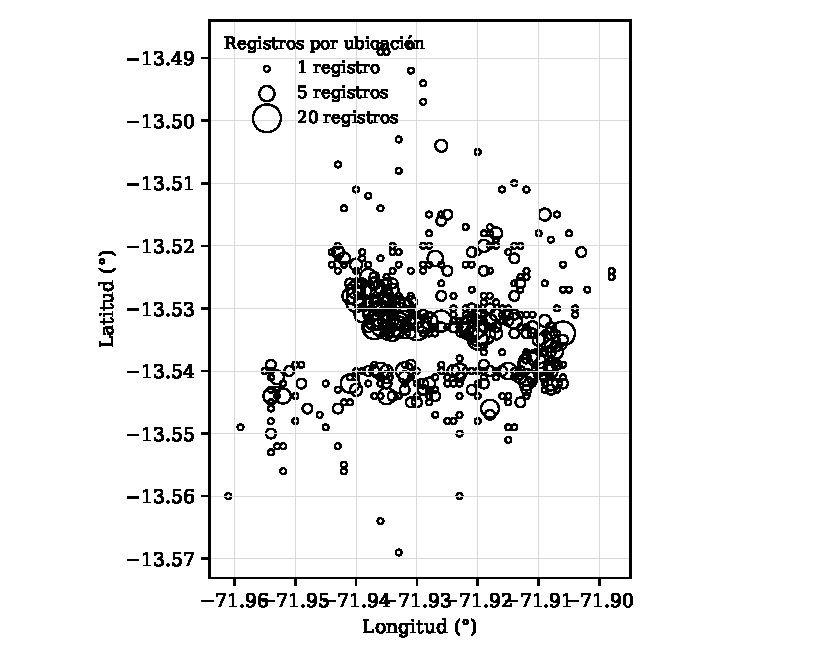
\includegraphics[width=0.72\textwidth]{diag_ubicaciones.pdf}
\caption{Ubicaciones distintas del extracto SIPCOP Municipal (San Sebastián, 2025).}
\label{fig:ubicaciones}
\fuente{Elaboración propia a partir del CSV SIPCOP Municipal. El tamaño del círculo es proporcional al número de registros con esa coordenada; $n = 996$ registros en 412 ubicaciones. Generada con \texttt{datos/figuras\_diagnostico.py}.}
\end{figure}

\begin{figure}[H]
\centering
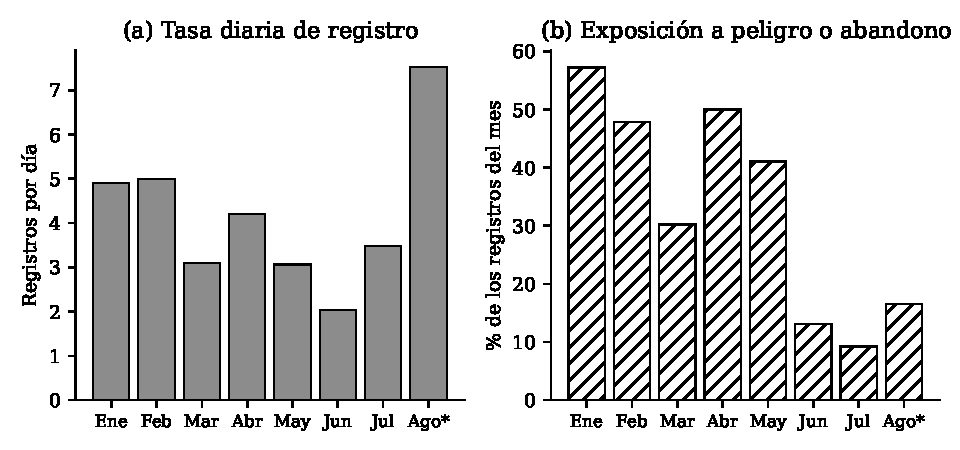
\includegraphics[width=0.95\textwidth]{diag_mensual.pdf}
\caption{Volumen de registro y modalidad de exposición a peligro o abandono por mes.}
\label{fig:mensual}
\fuente{Elaboración propia a partir del CSV SIPCOP Municipal. (*) Agosto incluye solo hasta el 29. En (a), la tasa es el número de registros dividido entre los días del mes observados; en (b), el porcentaje se calcula sobre los registros de cada mes.}
\end{figure}

\section{Técnicas e instrumentos de recolección}

\begin{itemize}
    \item \textbf{Análisis documental:} revisión del archivo CSV público de la capa SIPCOP Municipal para el distrito \texttt{080105}; se conservarán la URL de origen, fecha de descarga y archivo original para trazabilidad. Se solicitará a la municipalidad o al responsable de la capa la definición de los campos y del sistema de referencia espacial.
    \item \textbf{Instrumento:} ficha de estructura de datos (Anexo~\ref{anx:ficha}), que documenta las 19 columnas del archivo. Los campos analíticos son \texttt{fechaalerta}, \texttt{turno}, \texttt{especifico}, \texttt{modalidad}, \texttt{x} e \texttt{y}; se usan además \texttt{origen}, \texttt{naturalezadelpersonal}, \texttt{lugarocurrencia}, \texttt{consecuencia}, \texttt{formapatrullaje}, \texttt{direccion} y \texttt{tipovia} para la calidad de datos y los análisis de sensibilidad. El archivo no contiene una hora individual del hecho.
    \item \textbf{Cartografía:} polígono oficial del distrito y, si está disponible, la capa de manzanas o vías, para delimitar el área de simulación.
    \item \textbf{Herramientas de análisis:} Python con las bibliotecas \textit{pandas}, \textit{scikit-learn} \citep{pedregosa2011}, \textit{hdbscan} \citep{mcinnes2017} y \textit{SciPy}; un sistema de información geográfica para los mapas.
\end{itemize}

\section{Procedimiento metodológico}

\begin{enumerate}
    \item \textbf{Obtención y documentación.} Preservación del CSV disponible (996 registros; \texttt{id\_dist=080105}) y registro de su procedencia. Se consultará el significado de \texttt{fechaalerta}, los horarios de turno, las definiciones de categoría y la confirmación del sistema de referencia (el diagnóstico indica longitud y latitud en grados decimales, WGS84); cualquier autorización o validación municipal necesaria se gestionará antes de difundir resultados.
    \item \textbf{Depuración.} Revisión de duplicados, parseo de fechas, normalización de turnos y categorías, y comprobación de que las coordenadas correspondan al distrito. Se calculará la proporción de registros utilizables (objetivo específico~1) y se documentarán exclusiones.
    \item \textbf{Validación espacial.} Se verificará que \texttt{x} sea longitud e \texttt{y} latitud y que el sistema de referencia sea WGS84. Además se revisarán tres aspectos: (i) la cuantización a 0,001° y los ceros finales omitidos (126 valores de \texttt{x} y 145 de \texttt{y} tienen solo dos decimales); (ii) el contraste entre \texttt{direccion} y las coordenadas, usando puntos de referencia reconocibles (paraderos, el cementerio, el centro de salud); y (iii) la superposición con el polígono oficial del distrito. Solo después se transformarán a un sistema proyectado métrico o se usará haversine; si no se logra confirmar la referencia, no se interpretarán distancias ni agrupamientos métricos.
    \item \textbf{Análisis exploratorio.} Series por mes, día de la semana y turno dentro del periodo disponible; mapa de puntos y de densidad kernel (solo como visualización).
    \item \textbf{Agrupamiento espacial.} Se aplica DBSCAN con distancia haversine (Algoritmo~\ref{alg:dbscan}) y se elige la configuración según la regla de la sección~\ref{sec:parametros}. HDBSCAN se ejecuta como comparación.
    \item \textbf{Contraste de la concentración espacial.} Prueba Monte Carlo por grupo frente a aleatoriedad espacial completa (sección~\ref{sec:montecarlo}); los grupos significativos son los \textit{hotspots}.
    \item \textbf{Análisis temporal de los \textit{hotspots}.} Contrastes chi-cuadrado por turno, día de la semana y mes (sección~\ref{sec:temporal}).
    \item \textbf{Validación y presentación.} Revisión de los \textit{hotspots} con el personal del patrullaje municipal y elaboración de mapas.
\end{enumerate}

\algtitulo{DBSCAN aplicado a las ocurrencias georreferenciadas.}\label{alg:dbscan}
\noindent\textbf{Algoritmo \thealgoritmo.} DBSCAN aplicado a las ocurrencias georreferenciadas.
\begin{enumerate}
  \item Inicializar $C \gets 0$ y marcar todos los puntos como no visitados.
  \item Para cada punto $p \in D$ no visitado: marcarlo como visitado y calcular su vecindario $N_{\varepsilon}(p)$ con la distancia $d$ (ecuación~\ref{eq:haversine}).
  \item Si $|N_{\varepsilon}(p)| < \mathrm{MinPts}$, etiquetar $p$ como ruido.
  \item En caso contrario, crear un nuevo grupo $C$, asignar $p$ a dicho grupo y expandirlo con todos los puntos alcanzables dentro del radio $\varepsilon$.
  \item Repetir hasta que todos los puntos queden etiquetados como pertenecientes a un grupo o como ruido.
\end{enumerate}

\section{Protocolo de evaluación}

\subsection{Selección de parámetros y calidad del agrupamiento}
\label{sec:parametros}

La regla de selección se fija antes de ver los resultados de los contrastes. Las coordenadas tienen resolución de 0,001° (unos 108--111 m): dos puntos de celdas distintas distan al menos ese paso, de modo que con $\varepsilon \leq 100$ m solo se agrupan registros con coordenada idéntica, y $\varepsilon = 50$ y $100$ m producen la misma partición (diagnóstico preliminar). Por ello se explora una rejilla de $\varepsilon \in \{150, 200, 250, 300\}$ m y $\mathrm{MinPts} \in \{10, 20, 30\}$, y el gráfico de $k$-distancias orienta el rango de $\varepsilon$. Los registros con coordenadas idénticas cuentan como puntos separados al evaluar MinPts. Para cada configuración se calculan el número de grupos, el porcentaje de ruido y la silueta media (ecuación~\ref{eq:silueta}) sobre los puntos asignados. Se elige la configuración con mayor estabilidad, medida como el índice de Rand ajustado promedio (ARI) \citep{hubert1985} entre sus asignaciones y las de las configuraciones vecinas de la rejilla, entre las que tengan al menos dos grupos, menos de 60\,\% de ruido y ningún grupo que reúna más de 25\,\% de los registros depurados o supere 1 km de diámetro, para que no domine un grupo único formado por encadenamiento. La silueta no decide la elección y se interpreta con cautela, porque los puntos coincidentes (distancia cero) y la malla de coordenadas la distorsionan. Se presentará además el análisis de sensibilidad con las demás configuraciones.

\subsection{Comparación entre DBSCAN y HDBSCAN}

Se compararán las asignaciones de ambos algoritmos mediante el ARI, el número de grupos, el porcentaje de ruido y la coincidencia de los grupos grandes (los centroides a menos de $\varepsilon$ de distancia). Para HDBSCAN se variará el tamaño mínimo de grupo en un rango análogo a MinPts. La comparación es descriptiva: no se declara un algoritmo ``correcto'', sino en qué zonas coinciden y en cuáles difieren.

\subsection{Concentración espacial frente al azar}
\label{sec:montecarlo}

El modelo nulo de referencia es la aleatoriedad espacial completa (CSR): $n$ puntos independientes y uniformes dentro del \textbf{polígono real del distrito}, con el mismo $n$ que los datos depurados. La CSR es la referencia mínima, no un contraste exigente: casi cualquier ciudad rechaza la uniformidad porque la población, las vías y el comercio no se reparten de manera uniforme. Por eso se añade un \textbf{segundo modelo nulo}: la simulación restringida al área urbanizada (manzanas o vías) y, para los análisis por tipo de ocurrencia, la simulación con intensidad proporcional a la densidad kernel de todas las ocurrencias del extracto (de modo que se pregunte si un tipo se concentra más que el conjunto). Se informan los resultados bajo ambos nulos.

Se simulan $B = 999$ conjuntos y a cada uno se le aplica el agrupamiento con los parámetros ya elegidos para los datos reales, tras redondear las coordenadas simuladas a la misma rejilla de 0,001°; de lo contrario los datos reales parecerían más densos que el azar solo por la cuantización. El estadístico es el tamaño $m_j$ de cada grupo observado $j$. Su valor $p$ se calcula contra el tamaño del mayor grupo de cada simulación, $M_b$, lo que controla el error en las comparaciones entre grupos:
\begin{equation}
p_{j} = \frac{1 + \#\{\, b : M_b \geq m_j \,\}}{1 + B}
\label{eq:montecarlo}
\eqtitulo{Valor $p$ Monte Carlo de un grupo espacial.}
\end{equation}
Un grupo con $p_j < \alpha$ se considera un \textit{hotspot}. La comparación global (número de puntos en grupos frente a lo simulado) se informa como apoyo para $H_1$. Esta prueba se limita a comparar con una distribución uniforme: no distingue entre concentración por mayor actividad delictiva y concentración por mayor población, vías o presencia de patrullaje.

\subsection{Distribución temporal de los \textit{hotspots}}
\label{sec:temporal}

Para cada \textit{hotspot} se compara la distribución de sus ocurrencias según fecha de alerta (día de la semana y mes) y turno con la del resto del distrito, es decir, con las ocurrencias que no pertenecen a ese \textit{hotspot}. La referencia principal es la prueba chi-cuadrado de homogeneidad (ecuación~\ref{eq:chi2}) sobre la tabla de contingencia \textit{hotspot} frente a resto por categoría temporal; cuando más del 20\,\% de las frecuencias esperadas sea menor que 5 se usa una prueba de permutación \citep{cochran1954}. Esta referencia absorbe la variación del volumen de registro entre meses, que es grande en el extracto (de 2,0 registros diarios en junio a 7,5 en agosto) y que no se debe a ningún \textit{hotspot} en particular.

Como \textbf{análisis secundario} se contrasta, mediante chi-cuadrado de bondad de ajuste, si cada \textit{hotspot} sigue la distribución esperada por exposición calendario:
\begin{itemize}
    \item \textbf{Turno:} proporcional a las horas de cada turno según la organización real del patrullaje (se pedirá a la municipalidad).
    \item \textbf{Día de la semana:} proporcional al número de veces que ocurre cada día calendario entre el 1 de enero y el 29 de agosto de 2025.
    \item \textbf{Mes:} proporcional al número de días observados de cada mes, incluidos enero y agosto parciales.
\end{itemize}
Como la tasa mensual de registro cambia tanto, esta referencia se rechazará casi con seguridad aun sin concentración espacial alguna; se informa pero no sustenta por sí sola H\textsubscript{2}. Además, 26 de los 241 días no tienen registro y se desconoce si hubo cero eventos o falta de reporte; los contrastes se repiten sobre días con registro y sobre todos los días. El cambio de clasificación de ``exposición a peligro o abandono'' entre meses se controla repitiendo los contrastes sin esa modalidad (sección~\ref{sec:sensibilidad}).

Los contrastes suponen un riesgo constante en el tiempo y no prueban causalidad. Para evaluar si los \textit{hotspots} difieren entre sí en su distribución temporal se usa además la prueba chi-cuadrado de independencia sobre la tabla \textit{hotspot} por categoría temporal, con el tamaño del efecto medido mediante el coeficiente V de Cramér:
\begin{equation}
V = \sqrt{\frac{\chi^{2}}{n\,\min(r-1,\,c-1)}}
\label{eq:cramer}
\eqtitulo{Coeficiente V de Cramér.}
\end{equation}
donde $n$ es el total de ocurrencias y $r$ y $c$ el número de filas y de columnas de la tabla de contingencia.

\subsection{Análisis de sensibilidad}
\label{sec:sensibilidad}

Los resultados principales se repiten en cuatro variantes para valorar su robustez: (i) solo registros de origen ciudadano o de alarma (teléfono, alarma y mensajería; 232 registros), que dependen menos de dónde patrulla el personal; se declara de antemano que, por ser pocos registros, solo admitirán valores bajos de MinPts; (ii) el conjunto de presuntos delitos, sin la modalidad de exposición a peligro o abandono, por su cambio de clasificación entre meses; (iii) sin los 70 casi duplicados (misma fecha, turno y coordenadas); y (iv) con un desplazamiento aleatorio uniforme de $\pm 55$ m en las coordenadas, que aproxima el error por redondeo. Una conclusión se considera robusta solo si se mantiene en la mayoría de las variantes.

\section{Métodos de análisis de datos}

Se emplea estadística descriptiva (frecuencias, porcentajes, medidas de tendencia central) y las pruebas descritas arriba, con $\alpha = 0{,}05$. Como se contrastarán varios \textit{hotspots} y tres variables temporales, los valores $p$ de los contrastes temporales se ajustarán por comparaciones múltiples (corrección de Holm). Se fijará la semilla aleatoria y se versionarán los \textit{scripts} para garantizar la reproducibilidad.

\section{Aspectos éticos y de gestión de datos}

El estudio utiliza registros administrativos disponibles públicamente y se ajustará a la Ley de Protección de Datos Personales \citep{ley29733} y a las condiciones de uso de la fuente. Se emplearán solo los campos necesarios (\texttt{fechaalerta}, \texttt{turno}, \texttt{especifico} o \texttt{modalidad}, coordenadas), sin nombres ni documentos personales. Antes de publicar resultados se confirmarán las condiciones de reutilización con la entidad responsable; los resultados se agregarán por grupo y los mapas evitarán identificar domicilios concretos. El archivo de trabajo se almacenará de forma segura y se utilizará únicamente con fines de investigación.

\chapter{Estudio de factibilidad}

\section{Enfoque adoptado}

El proyecto se apoya en datos que la municipalidad ya produce y en herramientas de código abierto, sin entrenar modelos complejos ni requerir equipamiento especializado. La factibilidad se analiza en sus dimensiones técnica, económica y operativa.

\section{Factibilidad técnica}

\subsection{Hardware y cómputo}

El volumen disponible (996 registros de un distrito para enero-agosto de 2025) es manejable en un computador personal de gama media. DBSCAN y la simulación Monte Carlo (999 repeticiones) son ejecutables en ese equipo en tiempos razonables.

\subsection{Datos}

El CSV SIPCOP Municipal ya está disponible y se realizó un diagnóstico preliminar (Tabla~\ref{tab:diagnostico}): los 996 registros no tienen valores nulos en fecha, turno, tipo ni coordenadas, las coordenadas están en grados decimales con resolución de unos 110 m (412 ubicaciones distintas) y el volumen de registro varía de 2,0 a 7,5 por día entre meses. Los riesgos principales son la interpretación de \texttt{fechaalerta}, la ausencia de un diccionario que defina el sistema de referencia de \texttt{x} e \texttt{y}, la definición de las categorías y el cambio de clasificación entre meses. Se mitigarán documentando la fuente, consultando a la entidad responsable en las primeras semanas (de lo que dependen la rejilla de $\varepsilon$ y la referencia temporal) y tratando la evaluación de calidad como primer resultado (objetivo específico~1). Si no se confirma la referencia espacial, se limitará el análisis a los resultados que no dependan de distancias.

\subsection{Herramientas y software}

Se emplearán Python y sus bibliotecas de ciencia de datos (\textit{pandas}, \textit{scikit-learn}, \textit{hdbscan}, \textit{SciPy}), un sistema de información geográfica de código abierto para los mapas y \LaTeX{} para la redacción. Todas son de uso libre.

\section{Factibilidad económica}

El presupuesto estimado (Tabla~\ref{tab:presupuesto}) asciende a S/~1\,220,00, compuesto por gastos de servicios, materiales y trámites; al no requerir hardware ni licencias adicionales, es asumible con recursos propios.

\section{Factibilidad operativa}

El extracto público permite iniciar el análisis sin esperar una nueva entrega de datos. Se procurará la colaboración de la Municipalidad Distrital de San Sebastián para validar las definiciones de los campos, los horarios de turno y, de ser posible, interpretar los \textit{hotspots}; también se verificarán las condiciones de reutilización y difusión. El estudio no implica intervención sobre personas ni trabajo de campo extenso.

\section{Viabilidad y sostenibilidad}

El procedimiento (depuración, agrupamiento, contraste temporal) es replicable sobre nuevos periodos de datos y en otros distritos, y el uso de herramientas libres favorece que la municipalidad lo mantenga. La principal condición de continuidad es que el registro conserve coordenadas válidas.

\chapter{Aspectos administrativos}

\section{Cronograma de actividades}

El proyecto se ejecuta en 16 semanas, entre el 19 de octubre de 2026 y el 7 de febrero de 2027. La Tabla~\ref{tab:cronograma} presenta el diagrama de Gantt.

\begin{table}[H]
\centering
\caption{Cronograma de actividades por semanas (octubre 2026 -- febrero 2027).}
\label{tab:cronograma}
\begingroup\singlespacing\scriptsize
\setlength{\tabcolsep}{2.2pt}
\newcommand{\x}{$\blacksquare$}
\begin{tabular}{@{}>{\raggedright\arraybackslash}p{5.2cm}*{16}{c}@{}}
\toprule
 & \multicolumn{2}{c}{Oct} & \multicolumn{5}{c}{Nov} & \multicolumn{4}{c}{Dic} & \multicolumn{4}{c}{Ene} & Feb \\
\textbf{Actividad} & 1 & 2 & 3 & 4 & 5 & 6 & 7 & 8 & 9 & 10 & 11 & 12 & 13 & 14 & 15 & 16 \\
\midrule
Aprobación del plan de tesis & \x & \x & & & & & & & & & & & & & & \\
Solicitud de autorización y acceso a datos & \x & \x & \x & \x & & & & & & & & & & & & \\
Reunión con la municipalidad (CRS, fecha de alerta, turnos, categorías) & \x & \x & & & & & & & & & & & & & & \\
Revisión del estado del arte & \x & \x & \x & \x & & & & & & & & & & & & \\
Depuración y georreferenciación & & & \x & \x & \x & & & & & & & & & & & \\
Control de calidad y ajuste del diseño (rejilla de $\varepsilon$, referencia temporal) & & & & & \x & \x & & & & & & & & & & \\
Análisis exploratorio & & & & & & \x & \x & & & & & & & & & \\
Agrupamiento espacial (DBSCAN/HDBSCAN) & & & & & & & \x & \x & \x & & & & & & & \\
Prueba Monte Carlo y contrastes temporales & & & & & & & & \x & \x & \x & \x & & & & & \\
Mapas y validación con el patrullaje municipal & & & & & & & & & & \x & \x & \x & & & & \\
Redacción del informe final & & & & & & & & & & & \x & \x & \x & \x & \x & \\
Sustentación & & & & & & & & & & & & & & & \x & \x \\
\bottomrule
\end{tabular}
\endgroup
\fuente{Elaboración propia. Cada columna es una semana; la semana 1 inicia el 19 de octubre de 2026.}
\end{table}

\section{Presupuesto y financiamiento}

La Tabla~\ref{tab:presupuesto} resume los recursos estimados, que serán financiados con recursos propios del tesista.

\begin{table}[H]
\centering
\caption{Presupuesto estimado del proyecto (soles).}
\label{tab:presupuesto}
\begingroup\singlespacing\footnotesize
\begin{tabular}{@{}p{3.0cm}p{7.6cm}r@{}}
\toprule
\textbf{Rubro} & \textbf{Descripción} & \textbf{Costo (S/)} \\
\midrule
Servicios & Acceso a Internet durante cuatro meses & 240,00 \\
Materiales & Papel, impresiones y anillado de ejemplares & 300,00 \\
Trámites & Inscripción, derechos y trámites administrativos de la tesis & 400,00 \\
Movilidad & Traslados a la Municipalidad Distrital y a reuniones con el asesor & 180,00 \\
Imprevistos & Gastos no previstos & 100,00 \\
\midrule
\multicolumn{2}{@{}l}{\textbf{Total}} & \textbf{1\,220,00} \\
\bottomrule
\end{tabular}
\endgroup
\fuente{Elaboración propia. Los montos son estimaciones y se actualizarán con las tarifas vigentes.}
\end{table}

\section{Equipo de investigación}

\begin{table}[H]
\centering
\caption{Equipo de investigación.}
\label{tab:equipo}
\begingroup\singlespacing\footnotesize
\begin{tabular}{@{}p{2.6cm}p{11.5cm}@{}}
\toprule
\textbf{Rol} & \textbf{Responsable y función} \\
\midrule
Tesista & Br. Ronaldo Ticona Jancco: diseño, ejecución del análisis y redacción. \\
Asesor & Por designar: orientación metodológica y técnica. \\
Colaboradores & Personal de la Municipalidad Distrital de San Sebastián (acceso a datos y validación de los \textit{hotspots}). \\
\bottomrule
\end{tabular}
\endgroup
\fuente{Elaboración propia.}
\end{table}


\clearpage
\phantomsection
\addcontentsline{toc}{chapter}{Referencias}
\printbibliography[title={Referencias}]

\anexo{Matriz de consistencia}
\label{anx:matriz}

\begin{table}[H]
\centering
\caption{Matriz de consistencia.}
\label{tab:consistencia}
\begingroup\singlespacing\footnotesize
\begin{tabular}{@{}p{3.4cm}p{3.7cm}p{3.7cm}p{3.3cm}@{}}
\toprule
\textbf{Problema} & \textbf{Objetivo} & \textbf{Hipótesis} & \textbf{Técnica} \\
\midrule
General: ¿cuáles son los patrones de distribución espacial y temporal de las ocurrencias del extracto SIPCOP Municipal de San Sebastián, del 1/1 al 29/8 de 2025? & Analizar la distribución espacial y temporal del extracto mediante técnicas de agrupamiento y procedimientos estadísticos & H\textsubscript{G} (sección~\ref{sec:hipotesis}) & Agrupamiento espacial y análisis temporal \\
\addlinespace
PE1: proporción de ocurrencias utilizables, resolución espacial y convención de georreferenciación & OE1: evaluar la calidad y cobertura de los registros del SIPCOP-M y caracterizar la resolución de las coordenadas & Descriptivo (sin hipótesis) & Depuración, diagnóstico y georreferenciación \\
\addlinespace
PE2: concentraciones espaciales, cuáles superan el azar y coincidencia con HDBSCAN & OE2: identificar y contrastar las concentraciones con DBSCAN y compararlas con HDBSCAN & H\textsubscript{1} & DBSCAN ($\varepsilon$ de 150 a 300 m), HDBSCAN, ARI y prueba Monte Carlo con dos modelos nulos (CSR y área urbanizada) \\
\addlinespace
PE3: distribución temporal de los \textit{hotspots} frente al resto del distrito (y, como análisis secundario, frente a la exposición calendario) & OE3: analizar la distribución temporal de los \textit{hotspots} & H\textsubscript{2} & Chi-cuadrado de homogeneidad o permutación, V de Cramér, Holm y análisis de sensibilidad \\
\bottomrule
\end{tabular}
\endgroup
\fuente{Elaboración propia.}
\end{table}

\anexo{Ficha de estructura de datos del SIPCOP-M}
\label{anx:ficha}

\begingroup\singlespacing\footnotesize
\begin{longtable}{@{}p{4.0cm}>{\raggedright\arraybackslash}p{1.9cm}>{\raggedright\arraybackslash}p{5.3cm}>{\raggedright\arraybackslash}p{3.0cm}@{}}
\caption{Campos del archivo CSV SIPCOP Municipal (19 columnas).}\label{tab:ficha}\\
\toprule
\textbf{Campo del CSV} & \textbf{Tipo} & \textbf{Descripción observada} & \textbf{Uso previsto} \\
\midrule
\endfirsthead
\toprule
\textbf{Campo del CSV} & \textbf{Tipo} & \textbf{Descripción observada} & \textbf{Uso previsto} \\
\midrule
\endhead
\bottomrule
\endfoot
\texttt{fechaalerta} & Texto (fecha) & Fecha de alerta en español (``agosto 23, 2025''); semántica por confirmar & Día de semana, mes; conversión a fecha \\
\texttt{turno} & Categórica & Mañana, tarde, noche & Análisis temporal \\
\texttt{especifico} & Categórica & 8 categorías (vida, cuerpo y salud; patrimonio; etc.) & Descripción, conjuntos por tipo \\
\texttt{modalidad} & Categórica & Modalidad presunta (por ejemplo, exposición a peligro o abandono, robo a personas) & Conjunto de presuntos delitos \\
\texttt{generico} & Categórica & Valor único: alertas tempranas en apoyo a la PNP & Delimita el extracto \\
\texttt{origen} & Categórica & Patrullaje, teléfono, alarma, WhatsApp, cámara, operativo, otros & Sensibilidad por origen \\
\texttt{naturalezadelpersonal} & Categórica & Patrullaje Local Integrado o Patrullaje Municipal -- Serenazgo & Descripción y terminología \\
\texttt{formapatrullaje} & Categórica & Motorizado, a pie, bicicleta, otros & Descripción \\
\texttt{lugarocurrencia} & Categórica & Vía pública, inmueble particular, otros; 22\,\% faltante & Calidad de datos \\
\texttt{resultadoocurrencia} & Categórica & Consumado o frustrado; 67\,\% faltante & Calidad de datos \\
\texttt{consecuencia} & Categórica & Ninguno, materiales, lesiones, etc.; 10\,\% faltante & Calidad de datos \\
\texttt{medioutilizado} & Categórica & 32\,\% faltante y 64\,\% ``OTROS'' & Calidad de datos \\
\texttt{tipovia} & Categórica & Calle, avenida, pasaje, jirón; 175 ``SIN DATO'' & Descripción \\
\texttt{direccion} & Texto libre & Dirección o punto de referencia; 5 ``SIN DATO'' & Contraste con coordenadas \\
\texttt{estado}, \texttt{estadoocurrencia} & Categórica & \texttt{estado} constante (activo); casi todos cerrados & Verificación \\
\texttt{id\_dist} & Código & 080105 en todo el extracto & Verificación del ámbito \\
\texttt{x} & Numérica (texto) & Longitud en grados decimales, 3 decimales (unos 108 m) & Análisis espacial tras validar \\
\texttt{y} & Numérica (texto) & Latitud en grados decimales, 3 decimales (unos 111 m) & Análisis espacial tras validar \\
\end{longtable}
\endgroup
\fuente{Campos observados en el CSV disponible (separador \texttt{;}, codificación UTF-8 con BOM, saltos de línea CRLF, coordenadas entre comillas). La definición de categorías, el significado de la fecha de alerta y el sistema de referencia se confirmarán con la entidad responsable.}

\anexo{Registro de depuración de datos}
\label{anx:depuracion}

\begin{table}[H]
\centering
\caption{Registro de depuración preliminar.}
\label{tab:depuracion}
\begingroup\singlespacing\footnotesize
\begin{tabular}{@{}p{7.0cm}p{3.0cm}p{3.0cm}@{}}
\toprule
\textbf{Etapa} & \textbf{Registros restantes} & \textbf{Registros excluidos} \\
\midrule
Registros del CSV disponible (1/1--29/8/2025) & 996 & --- \\
Tras eliminar duplicados exactos & 986 & 10 \\
Con \texttt{fechaalerta} y turno válidos & 986 & 0 \\
Con coordenadas presentes y parseables & 986 & 0 \\
Con CRS validado y ubicación dentro del distrito & Por completar & Por completar \\
\textbf{Registros utilizables para el análisis} & Por completar (máximo 986) & Por completar \\
\bottomrule
\end{tabular}
\endgroup
\fuente{Conteos del diagnóstico preliminar. Los 70 registros con igual fecha, turno y coordenadas no se excluyen (ver sección~3.3.2). Falta verificar la ubicación frente al polígono distrital.}
\end{table}


\end{document}
